\chapter{Conclusion}\label{chapter: conclusion}

In this final chapter, we want to recap the languages and frameworks about their abilities and provided functionality.

\begin{tabular}{l |c |c |c |c }
	Property 						& \cnnarch 		& \caffe 		& \caffetwo 		& \mxnet \\ \hline
					\multicolumn{5}{c}{General Information}\\\hline
	is full framework  				& \xmark		& \cmark		& \cmark			& \cmark \\
	SLI usage						& (\cmark)$^5$	& \xmark$^1$ 	& \xmark$^1$ 		& \cmark \\
	mult. computers 				& (\cmark)$^5$	& \cmark		& \cmark			& \cmark \\	
	\hline
					\multicolumn{5}{c}{Nets Supported}\\ \hline
	typical CNNs					& \cmark		& \cmark		& \cmark			& \cmark \\
	arbitrary CNNs					& \xmark		& \cmark		& \cmark			& \cmark \\
	Recurrent NNs					& \xmark		& \cmark		& \cmark			& \cmark \\
	\hline
					\multicolumn{5}{c}{Constructs}\\ \hline
	predefined NNs					& \cmark		& \cmark		& \cmark			& \cmark \\
	pre-trained NNs  				& \xmark		& \cmark		& \xmark$^2$		& \cmark \\
	arbitrary net creation			& \cmark		& \xmark 		& \xmark			& \cmark \\	
	predefined functions 		  	& \cmark		& \cmark		& \cmark			& \cmark \\
	simple function creation 	  	& \cmark 		& \xmark		& \xmark$^2$		& \cmark \\
	low-level operations			& \xmark		& \xmark		& \xmark			& \cmark \\ %check
	\hline
					\multicolumn{5}{c}{Language bindings}\\ \hline
	C++								& \xmark		& \cmark$^3$	& \cmark			& \cmark \\
	Python							& \cmark		& \cmark$^3$	& \cmark			& \cmark \\
	MATLAB							& \xmark$^2$	& \cmark$^3$	& \xmark			& \cmark \\ 
	Others							& --			& Apache Spark$^4$& --				& R, Go, Julia, Perl\\
									&				&				&					& JavaScript, Scala \\ 
%	\hline
%					\multicolumn{5}{c}{Usage}\\ \hline
%					understandability & & & & \\
%					handling & & & & \\
\end{tabular}

\vspace{-1em}
\begin{figure}[H]
	\footnotesize
	\begin{multicols}{2}
	\begin{itemize}
		\item[$^1$] CUDA does not generally support SLI
		\item[$^2$] not clearly stated, but also not denied
		\item[$^3$] nets still written in prototxt (c.f. \Cref{sec: Caffe})
		\item[$^4$] made by a third party\cite{CaffeOnSpark}
		\item[$^5$] through the usage of \mxnet
	\end{itemize}
	\end{multicols}
\end{figure}

Overall, we can conclude that \cnnarch has the potential to become a recognized domain specific language for deep learning. The python like syntax and simplistic way of defining a net is superior to the protocol buffer approach of \caffe. Since \cnnarch is not a full framework, but compiles its code to \mxnet code, it benefits from MxNets ability of SLI and even cluster usage. The possibility to define recurrent \nns is still up to be implemented. An example of a \nn that can not be implemented in \cnnarch can be seen in \Cref{pic: Simple RNN}. There a neuron is connected to itself in order to use the latest value it outputted. In order to improve the reputation \cnnarch and to enlarge the community a library of pre-trained models would be desirable.

\begin{figure}
	\centering
	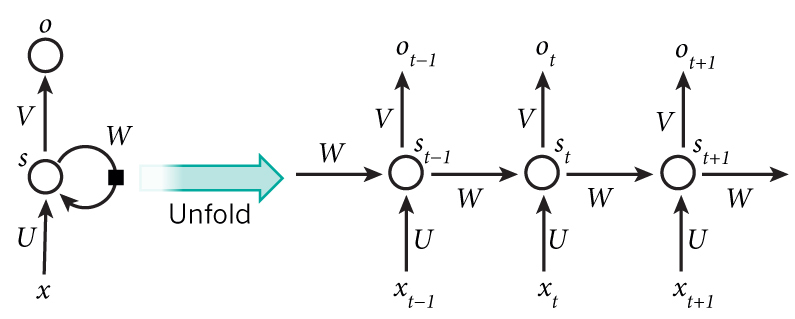
\includegraphics[scale=0.3]{src/pic/rnn.jpg}
	\caption{A single recurrent connection and its semantical interpretation \cite{britz2015recurrent}.}
	\label{pic: Simple RNN}
\end{figure}

Summarizing, the most important aspect of state-of-the-art deep learning frameworks is the efficiency. Through various methods and researches like \kitti and \torcs the data to train a network is available.\\
Also to mention is the data estimation in \cite{grzywaczewski2017training}. There, a fleet of 100 cars is analyzed based on how much useful data is produced during one year. After conservative preprocessing this leads to 104 TB of data, which would take an \alexnet roughly $1.2$ years to train, if only a single GPU is used. The possibility of using multiple machines is a key element. Using 18 DGX-1 Volta systems, the same effort of training can be done within seven days.
